\section*{Теория}

\textit{Центрированными оптическими системами} называются отражающие и преломляющие однородные среды, отделённые сферическими поверхностями, центры кривизны которых лежат на лежат на одной прямой, называемой \textit{главной оптической осью}.

Пучки света называются \textit{гомоцентрическими}, если выйдя из точки и пройдя оптическую систему, они сходятся в точке.

Оптическая система называется \textit{идеальной}, если пучки гомоцентрические и изображение подобно предмету. Идеальная оптическая система реализуется оптической системой в параксиальном приближении.

Рассмотрим элементарную оптическую ячейку, состоящую из преломляющей сферической поверхности, разделяющей однородные среды с показателями преломления $n$ и $n'$:

\begin{figure}[H]
	\centering
	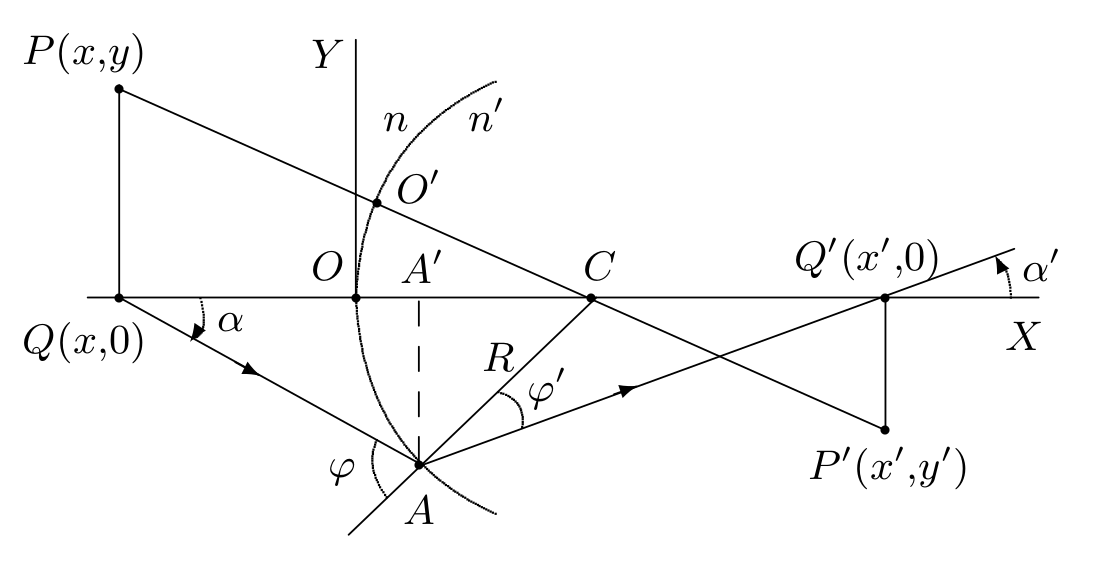
\includegraphics[width=0.5\textwidth]{../Изображения/Оптическая ячейка.png}
\end{figure}

Начало координат поместим в точку $O$ -- точку пересечения преломляющей поверхности и главной оптической оси. Расстояние до предмета обозначим как $x$, расстояние до изображения $x'$. Расстояния положительны, если направление распространения луча совпадает с направлением отсчёта. Поперечный размер предмета обозначим как $y$, изображения как $y'$. Размер будем считать положительным, если предмет находится выше главной оптической оси, отрицательным, если ниже. Радиусы кривизны отсчитываются от поверхности к центру кривизны.

Для элементарной оптической ячейки в параксиальном приближении выполняется соотношение:
$$- \frac{n}{x} + \frac{n'}{x'} = \frac{n' - n}{R}$$
$$x \alpha = x' \alpha'$$
Из полученных соотношений видно, что все лучи выходящие из одной точки главной оптической оси, после преломления на сферической поверхности пересекутся примерно в одной точке на главной оптической оси.
